\documentclass[aspectratio=169,10pt]{beamer}
\usetheme{default}
\usepackage[utf8]{inputenc}
\usepackage[T1]{fontenc}
\usepackage{lmodern}
\usepackage{graphicx}
\usepackage{booktabs}
\usepackage{listings}
\usepackage{pgfplots}
\usepackage{etoolbox}
\pgfplotsset{compat=1.16}
\graphicspath{{docs/assets/figures/}{docs/assets/screens/}}

\setbeamercolor{normal text}{fg=black,bg=white}
\setbeamertemplate{navigation symbols}{}
\setbeamertemplate{footline}[frame number]
\setbeamertemplate{itemize items}[circle]
\setbeamerfont{block title}{size=\footnotesize,series=\bfseries}
\setbeamerfont{block body}{size=\footnotesize}
\setbeamerfont{itemize/enumerate body}{size=\footnotesize}
\setbeamerfont{itemize/enumerate subbody}{size=\scriptsize}
\setbeamerfont{frametitle}{size=\large,series=\bfseries}
\AtBeginEnvironment{tabular}{\footnotesize}
\newcommand{\code}[1]{\texttt{\footnotesize #1}}
\newcommand{\fig}[2]{\includegraphics[#1]{#2}}
\renewcommand{\arraystretch}{1.12}

\lstdefinestyle{code}{basicstyle=\fontsize{7.2}{8.6}\selectfont\ttfamily,breaklines=true,breakatwhitespace=false,
  frame=single,rulecolor=\color{black!40},numbers=left,numberstyle=\tiny\color{black!55},numbersep=5pt,
  showstringspaces=false,columns=fullflexible,keepspaces=true,xleftmargin=1.6em,framexleftmargin=1.4em,aboveskip=0pt,belowskip=0pt}
\lstdefinestyle{term}{style=code,numbers=none,xleftmargin=0pt,framexleftmargin=0pt,basicstyle=\fontsize{7}{8.3}\selectfont\ttfamily}
% a source excerpt, a terminal capture, and a slide made of one of each
\newcommand{\listing}[1]{\lstinputlisting[style=code,firstnumber=1]{docs/assets/listings/#1.txt}}
\newcommand{\terminal}[1]{\lstinputlisting[style=term]{docs/assets/listings/#1.txt}}
\newcommand{\listingr}[3]{\lstinputlisting[style=code,firstline=#2,lastline=#3,firstnumber=#2]{docs/assets/listings/#1.txt}}
\newcommand{\terminalr}[3]{\lstinputlisting[style=term,firstline=#2,lastline=#3]{docs/assets/listings/#1.txt}}

\title{Semantic Log Analytics [UAV Log]}
\subtitle{UAV flight logs as a database problem: time series, semantics, search and guarded SQL}
\author{Sumit Kumar (22CS30056)}
\institute{Advanced Database Management Systems (CS60113), term project}
\date{\footnotesize github.com/SumitKumar-17/UAVLog}

\newcommand{\pgfaxis}[1]{\begin{axis}[width=\linewidth,height=0.5\textheight,#1,grid=major,grid style={black!12},tick label style={font=\scriptsize},label style={font=\footnotesize},legend style={font=\tiny,at={(0.5,-0.28)},anchor=north,legend columns=3},cycle list={{blue!70!black,mark=*},{red!75!black,mark=square*},{green!45!black,mark=triangle*},{orange!85!black,mark=diamond*},{violet,mark=pentagon*}},every axis plot/.append style={thick,mark size=1.6pt}]}

\begin{document}

\begin{frame}[plain]\titlepage\end{frame}

% =============================================================== 1. problem
\begin{frame}[shrink=5]{Motivation: flight logs are a database problem}
\begin{columns}[T]
\begin{column}{0.49\textwidth}
\begin{block}{Three kinds of data at once}
\begin{itemize}
  \item \textbf{Time series}: 300 PX4 flights hold \textbf{70.7 M} telemetry samples
  \item \textbf{Text}: 3,401 events (warnings, failure flags, mode changes)
  \item \textbf{Vendor dialects}: PX4 and ArduPilot name the same quantity differently
\end{itemize}
\end{block}
\end{column}
\begin{column}{0.49\textwidth}
\begin{block}{What people need}
\begin{itemize}
  \item Questions across many flights, asked in words: \emph{``which flights lost a motor?''}
  \item Existing tools plot \textbf{one log at a time}
  \item Answers that are exact, explainable, and safe to run on the data
\end{itemize}
\end{block}
\end{column}
\end{columns}
\end{frame}

\begin{frame}[shrink=5]{Research questions and contributions}
\begin{columns}[T]
\begin{column}{0.49\textwidth}
\begin{block}{Four questions, each answered by an experiment}
\begin{itemize}
  \item \textbf{RQ1} How should high-rate telemetry be stored, and at what cost?
  \item \textbf{RQ2} Which vector index and filtering strategy retrieve events best?
  \item \textbf{RQ3} Can a model write safe, correct SQL; what does a semantic layer add?
  \item \textbf{RQ4} Do the event detectors find faults of known size?
\end{itemize}
\end{block}
\end{column}
\begin{column}{0.49\textwidth}
\begin{block}{Contributions}
\begin{itemize}
  \item One PostgreSQL schema for telemetry, ontology, events and embeddings
  \item A measured columnstore design and engine comparison
  \item A self-routing hybrid search and a filtered-search study
  \item A four-layer guarded NL-to-SQL with a measured evaluation
\end{itemize}
\end{block}
\end{column}
\end{columns}
\end{frame}

\begin{frame}[shrink=5]{Background: TimescaleDB}
\begin{columns}[T]
\begin{column}{0.49\textwidth}
\begin{block}{Concepts}
\begin{itemize}
  \item \textbf{Hypertable}: one logical table cut into time \emph{chunks}
  \item \textbf{Columnstore}: old chunks stored column-wise and compressed, grouped by \code{segmentby} and sorted by \code{orderby}
  \item \textbf{Continuous aggregate}: incrementally maintained rollup (here min, max, mean per second)
\end{itemize}
\end{block}
\end{column}
\begin{column}{0.49\textwidth}
\begin{block}{Why it fits telemetry}
\begin{itemize}
  \item Slowly changing sensor values compress to a few bytes
  \item Queries for one signal of one flight read one compressed segment, not the table
  \item Postgres features stay: SQL, joins, transactions, roles
\end{itemize}
\end{block}
\end{column}
\end{columns}
\end{frame}

\begin{frame}[shrink=5]{Background: vector search in Postgres}
\begin{columns}[T]
\begin{column}{0.49\textwidth}
\begin{block}{Index families}
\begin{itemize}
  \item \textbf{HNSW}: layered proximity graph; hop toward the query
  \item \textbf{IVFFlat}: sort vectors into clusters; probe the nearest few
  \item \textbf{DiskANN} (pgvectorscale): compressed graph built for disk
  \item Quality measure: \textbf{recall@k} against exact search
\end{itemize}
\end{block}
\end{column}
\begin{column}{0.49\textwidth}
\begin{block}{The filtering pitfall}
\begin{itemize}
  \item The index finds neighbours \textbf{first}; the SQL filter is applied \textbf{after}
  \item A selective filter can leave fewer rows than requested
  \item Remedies: iterative scan, exact sort, partial indexes, partitions (all measured here)
\end{itemize}
\end{block}
\end{column}
\end{columns}
\end{frame}

\begin{frame}[shrink=5]{The gap and the architecture}
\begin{columns}[T]
\begin{column}{0.36\textwidth}
\begin{block}{Gap in existing work}
\begin{itemize}
  \item Log viewers: one flight, no semantics
  \item Time-series stores: no ontology or vendor mapping
  \item NL-to-SQL demos: rarely guarded or measured
  \item To our knowledge no published system combines all three over PX4 logs
\end{itemize}
\end{block}
\end{column}
\begin{column}{0.62\textwidth}
\centering
\fig{width=\textwidth,height=0.65\textheight,keepaspectratio}{diagram-architecture.png}
\end{column}
\end{columns}
\end{frame}

\begin{frame}[shrink=5]{The data}
\begin{columns}[T]
\begin{column}{0.49\textwidth}
\begin{block}{Corpus}
\begin{itemize}
  \item 300 flights chosen (seeded, stratified) from 478,918 public Flight Review logs; CC-BY
  \item 8.75 GB of PX4 ULog files, parsed to a Parquet raw layer and the canonical telemetry table
  \item 70,731,891 telemetry rows, 3,401 events
\end{itemize}
\end{block}
\end{column}
\begin{column}{0.49\textwidth}
\begin{block}{Second autopilot}
\begin{itemize}
  \item An ArduPilot MAVLink log is ingested through the same ontology
  \item It shows the vendor mapping at work: one canonical signal name for both autopilots
  \item Gaps are documented, not guessed (see the semantic layer)
\end{itemize}
\end{block}
\end{column}
\end{columns}
\end{frame}

% =============================================================== platform tour
\begin{frame}[shrink=5]{The platform: what was built}
\begin{columns}[T]
\begin{column}{0.49\textwidth}
\begin{block}{Data and database}
\begin{itemize}
  \item One PostgreSQL with TimescaleDB (columnstore) and pgvector
  \item Ontology and canonical mapping for PX4 and ArduPilot
  \item 3,401 events, embeddings, flight signatures, signal windows
\end{itemize}
\end{block}
\begin{block}{Search and language}
\begin{itemize}
  \item Hybrid search with a self-routing filtered query
  \item Guarded natural-language SQL and cited incident reports
\end{itemize}
\end{block}
\end{column}
\begin{column}{0.49\textwidth}
\begin{block}{Application (Next.js and FastAPI)}
\begin{itemize}
  \item Flights, replay, similar moments, incident reports
  \item Map, fleet galaxy, incidents feed
  \item Ask, SQL workbench, data explorer, command palette
  \item Database and Benchmarks pages drawn from live data
\end{itemize}
\end{block}
\end{column}
\end{columns}
\end{frame}

\begin{frame}{Overview: entry points to every feature}
\centering
\fig{width=0.97\textwidth,height=0.8\textheight,keepaspectratio}{deck-overview-light-1440.png}\par\vspace{0.15em}
{\footnotesize Search by meaning, shortcuts to every feature, and flights ranked by critical events with a strip of flight modes for each.}
\end{frame}

\begin{frame}{Flights: every flight as a strip}
\centering
\fig{width=0.97\textwidth,height=0.8\textheight,keepaspectratio}{deck-flights-light-1440.png}\par\vspace{0.15em}
{\footnotesize Colour is the flight mode over time; marks are warnings and failures. Sort by critical events, recency or length.}
\end{frame}

\begin{frame}{One flight: modes, charts, track and events}
\centering
\fig{width=0.97\textwidth,height=0.8\textheight,keepaspectratio}{deck-flight-light-1440.png}\par\vspace{0.15em}
{\footnotesize The mode ribbon with event marks, a replay bar, synchronized charts, the ground track and the event list.}
\end{frame}

\begin{frame}{Behaviour strip: how unusual each 10 seconds were}
\centering
\fig{width=0.97\textwidth,height=0.8\textheight,keepaspectratio}{deck-flight-behaviour-light-1440.png}\par\vspace{0.15em}
{\footnotesize Every window is compared with its 5 nearest windows in other flights (one vector search each) and shown as a percentile of the whole corpus: blue typical, red unusual.}
\end{frame}

\begin{frame}{Why a window is unusual}
\centering
\fig{width=0.97\textwidth,height=0.8\textheight,keepaspectratio}{docs/assets/screens/deck-flight-why-light-1440.png}\par\vspace{0.15em}
{\footnotesize Click a window or one of the most unusual moments: the signal statistics furthest from the typical flight, in units of the typical spread, with the value and the corpus median.}
\end{frame}

\begin{frame}{Signal relationships}
\centering
\fig{width=0.97\textwidth,height=0.8\textheight,keepaspectratio}{docs/assets/screens/deck-flight-relations-light-1440.png}\par\vspace{0.15em}
{\footnotesize Pearson correlation of every pair of signals in the flight on a one-second grid: orange moved together, blue moved oppositely.}
\end{frame}

\begin{frame}{Synchronized charts with min/max envelopes}
\centering
\fig{width=0.97\textwidth,height=0.8\textheight,keepaspectratio}{deck-flight-signals-light-1440.png}\par\vspace{0.15em}
{\footnotesize Drag across any chart to zoom every chart together; envelopes keep short spikes visible when zoomed out.}
\end{frame}

\begin{frame}{Flight replay}
\centering
\fig{width=0.97\textwidth,height=0.8\textheight,keepaspectratio}{deck-flight-replay-light-1440.png}\par\vspace{0.15em}
{\footnotesize The time cursor sweeps the charts and the track at 1x to 64x, shows the current mode, and surfaces events as it passes them.}
\end{frame}

\begin{frame}{Incident report with citations}
\centering
\fig{width=0.97\textwidth,height=0.8\textheight,keepaspectratio}{deck-flight-report-light-1440.png}\par\vspace{0.15em}
{\footnotesize Numbered evidence is computed by SQL; the model writes prose and may only cite it; a citation jumps the charts to that moment.}
\end{frame}

\begin{frame}{Similar moments}
\centering
\fig{width=0.97\textwidth,height=0.8\textheight,keepaspectratio}{deck-flight-moments-light-1440.png}\par\vspace{0.15em}
{\footnotesize Pick a moment and find where, in other flights, the signals behaved the same way: 10-second window embeddings searched with HNSW.}
\end{frame}

\begin{frame}{Similar moments: overlay}
\centering
\fig{width=0.97\textwidth,height=0.8\textheight,keepaspectratio}{deck-flight-overlay-light-1440.png}\par\vspace{0.15em}
{\footnotesize Overlay draws the same signal over the two matching windows, so the similarity can be seen, not just a distance.}
\end{frame}

\begin{frame}{Semantic search}
\centering
\fig{width=0.97\textwidth,height=0.8\textheight,keepaspectratio}{deck-search-light-1440.png}\par\vspace{0.15em}
{\footnotesize Vector, full text and filters fused by reciprocal rank fusion, with the ranking details and the chosen filter strategy shown.}
\end{frame}

\begin{frame}{Ask: natural language to guarded SQL}
\centering
\fig{width=0.97\textwidth,height=0.8\textheight,keepaspectratio}{deck-ask-light-1440.png}\par\vspace{0.15em}
{\footnotesize The SQL that ran, the planner's cost estimate and every guard action are shown next to the answer.}
\end{frame}

\begin{frame}{Compare two flights}
\centering
\fig{width=0.97\textwidth,height=0.8\textheight,keepaspectratio}{deck-compare-light-1440.png}\par\vspace{0.15em}
{\footnotesize The same canonical signal from flights on different boards, aligned at takeoff, with event counts side by side.}
\end{frame}

\begin{frame}{Ontology}
\centering
\fig{width=0.97\textwidth,height=0.8\textheight,keepaspectratio}{deck-ontology-light-1440.png}\par\vspace{0.15em}
{\footnotesize Concepts, relations and the vendor fields mapped to them for both autopilots.}
\end{frame}

\begin{frame}{Map}
\centering
\fig{width=0.97\textwidth,height=0.8\textheight,keepaspectratio}{deck-map-light-1440.png}\par\vspace{0.15em}
{\footnotesize Every flight with a GPS fix, coloured by critical events and sized by length; filter by board; click to open.}
\end{frame}

\begin{frame}{Fleet galaxy}
\centering
\fig{width=0.97\textwidth,height=0.8\textheight,keepaspectratio}{deck-fleet-galaxy-light-1440.png}\par\vspace{0.15em}
{\footnotesize Each flight placed by how it behaved (signature PCA); colour by board, firmware, critical events or unusualness.}
\end{frame}

\begin{frame}{Fleet statistics}
\centering
\fig{width=0.97\textwidth,height=0.8\textheight,keepaspectratio}{deck-fleet-boards-light-1440.png}\par\vspace{0.15em}
{\footnotesize Critical events per flight by board and firmware, event kinds, flights per year and flight length.}
\end{frame}

\begin{frame}{A year of flying}
\centering
\fig{width=0.97\textwidth,height=0.8\textheight,keepaspectratio}{deck-fleet-calendar-light-1440.png}\par\vspace{0.15em}
{\footnotesize One square per day for the last 12 months: flights or critical events.}
\end{frame}

\begin{frame}{Incidents}
\centering
\fig{width=0.97\textwidth,height=0.8\textheight,keepaspectratio}{deck-incidents-light-1440.png}\par\vspace{0.15em}
{\footnotesize Every warning and failure across flights; filter by severity, kind, board and wording; open at the exact moment.}
\end{frame}

\begin{frame}{Upload a log}
\centering
\fig{width=0.97\textwidth,height=0.8\textheight,keepaspectratio}{docs/assets/screens/deck-upload-light-1440.png}\par\vspace{0.15em}
{\footnotesize Drop a PX4 .ulg file: it is validated (header, size, not a duplicate), queued like any other log and run through ingest, events, event embeddings, window embeddings and summaries, with each stage shown as it finishes (about 20 seconds for a 17 MB log).}
\end{frame}

\begin{frame}{Patterns: what happens before and after an event}
\centering
\fig{width=0.97\textwidth,height=0.8\textheight,keepaspectratio}{deck-patterns-light-1440.png}\par\vspace{0.15em}
{\footnotesize A windowed self-join of the event table: for each other kind, the share of flights in which it occurred within the window before or after, against its overall frequency (lift).}
\end{frame}

\begin{frame}{Signals: distributions across the corpus}
\centering
\fig{width=0.97\textwidth,height=0.8\textheight,keepaspectratio}{docs/assets/screens/deck-signals-light-1440.png}\par\vspace{0.15em}
{\footnotesize Every canonical signal with the distribution of its per-flight mean (SQL width\_bucket over the signal summary); click one for the flights with the highest and lowest values.}
\end{frame}

\begin{frame}{Rule lab: tune a detector}
\centering
\fig{width=0.97\textwidth,height=0.8\textheight,keepaspectratio}{docs/assets/screens/deck-rules-light-1440.png}\par\vspace{0.15em}
{\footnotesize Move a threshold and the rule is re-run over every flight, then scored against the autopilot's own warnings; precision, recall and F1 across the range, with the shipped threshold marked.}
\end{frame}

\begin{frame}{SQL workbench}
\centering
\fig{width=0.97\textwidth,height=0.8\textheight,keepaspectratio}{deck-workbench-light-1440.png}\par\vspace{0.15em}
{\footnotesize Write your own SQL under the same four checks as Ask; schema browser, saved queries, planner cost and the rebuilt SQL.}
\end{frame}

\begin{frame}{SQL workbench: the query plan}
\centering
\fig{width=0.97\textwidth,height=0.8\textheight,keepaspectratio}{deck-workbench-plan-light-1440.png}\par\vspace{0.15em}
{\footnotesize Explain shows the planner's plan as a tree with each node's share of the total cost and the cost limit used for admission; nothing is executed.}
\end{frame}

\begin{frame}{Data explorer: schema map}
\centering
\fig{width=0.97\textwidth,height=0.8\textheight,keepaspectratio}{deck-data-map-light-1440.png}\par\vspace{0.15em}
{\footnotesize The relations diagram, read live from the catalog; hover to follow foreign keys, click to browse a table.}
\end{frame}

\begin{frame}{Data explorer: browse rows}
\centering
\fig{width=0.97\textwidth,height=0.8\textheight,keepaspectratio}{deck-data-browse-light-1440.png}\par\vspace{0.15em}
{\footnotesize Every table and view with row counts and sizes; page through the rows, read-only.}
\end{frame}

\begin{frame}{Data explorer: structure}
\centering
\fig{width=0.97\textwidth,height=0.8\textheight,keepaspectratio}{deck-data-structure-light-1440.png}\par\vspace{0.15em}
{\footnotesize Columns, types, keys, indexes with sizes and, for the hypertable, the chunk and columnstore settings.}
\end{frame}

\begin{frame}{Performance: live database statistics}
\centering
\fig{width=0.97\textwidth,height=0.8\textheight,keepaspectratio}{docs/assets/screens/deck-performance-light-1440.png}\par\vspace{0.15em}
{\footnotesize Buffer cache hit ratio, connections, the costliest statements from pg\_stat\_statements, how tables are scanned and the settings that matter, refreshed every few seconds.}
\end{frame}

\begin{frame}[shrink=5]{Contents}
\begin{columns}[T]
\begin{column}{0.49\textwidth}
\begin{block}{Part 1: the platform}
\begin{itemize}
  \item What was built, and a tour of every feature
\end{itemize}
\end{block}
\begin{block}{Part 2: database design}
\begin{itemize}
  \item Schema, hypertable and columnstore design
  \item Storage results; TimescaleDB against DuckDB
\end{itemize}
\end{block}
\end{column}
\begin{column}{0.49\textwidth}
\begin{block}{Part 3: semantics and retrieval}
\begin{itemize}
  \item Ontology, events, fault injection
  \item Hybrid search, vector indexes, filtered search
\end{itemize}
\end{block}
\begin{block}{Part 4: language and evidence}
\begin{itemize}
  \item Guarded NL-to-SQL and its evaluation
  \item Database and benchmark pages; conclusions
\end{itemize}
\end{block}
\end{column}
\end{columns}
\end{frame}

\begin{frame}{Guided tour}
\centering
\fig{width=0.97\textwidth,height=0.8\textheight,keepaspectratio}{docs/assets/screens/deck-tour-light-1440.png}\par\vspace{0.15em}
{\footnotesize A Tour button in the top bar walks through every page with a card saying what to look at; Next, Back and the arrow keys move between pages.}
\end{frame}

% =============================================================== 2. schema
\begin{frame}[shrink=5]{Relational schema}
\centering
\fig{width=0.86\textwidth,height=0.46\textheight,keepaspectratio}{diagram-er.png}\par\vspace{0.3em}
\begin{columns}[T]
\begin{column}{0.49\textwidth}
\begin{itemize}
  \item \code{flight}: one row per log, parsed metadata
  \item \code{telemetry}: hypertable, one row per (time, flight, field)
  \item \code{vendor\_field}, \code{field\_mapping}: source field $\to$ concept with scale and offset
  \item \code{concept}, \code{concept\_relation}: ontology
\end{itemize}
\end{column}
\begin{column}{0.49\textwidth}
\begin{itemize}
  \item \code{event}: text, kind, time span, \code{vector(1536)}, generated \code{tsvector}
  \item \code{flight\_signature}: \code{vector(32)} signal-shape embedding
  \item \code{note}: investigation notes pinned to a time
  \item \code{llm\_call}: every model call with tokens, cost, latency
\end{itemize}
\end{column}
\end{columns}
\end{frame}

\begin{frame}{DDL: the telemetry hypertable}
\begin{block}{Narrow long format}
A new signal adds rows, never columns, and a new autopilot needs no schema change; the ontology maps vendor names to \code{vendor\_field\_id}. Seven-day chunks. As a plain rowstore the \textbf{index (7.6 GB) was larger than the table (4.9 GB)}.
\end{block}
\vspace{0.4em}
\listing{code-telemetry-ddl}
\end{frame}

\begin{frame}{Inspecting the hypertable: dimensions and columnstore settings}
\begin{block}{Reading}
One time dimension on \code{ts} with 7-day chunks, 134 chunks, columnstore enabled and segmented by flight and field, ordered by time.
\end{block}
\vspace{0.3em}
\terminal{term-hypertable}
\end{frame}

\begin{frame}{Inspecting the hypertable: chunks}
\begin{block}{Reading}
All chunks are compressed. The earliest ranges (1970, 2005) belong to logs whose device clock was implausible; the decision log (D6) describes how start times are guarded.
\end{block}
\vspace{0.3em}
\terminal{term-chunks}
\end{frame}

\begin{frame}{The event table, as the database reports it}
\terminalr{term-event}{1}{22}
\end{frame}

\begin{frame}{Indexes on the search tables}
\begin{block}{Reading}
One HNSW index on event embeddings (13 MB), one GIN index on the generated \code{tsvector}, B-trees for flight, kind and time filters, and a small HNSW index on flight signatures.
\end{block}
\vspace{0.4em}
\terminal{term-indexes}
\end{frame}

% =============================================================== 3. columnstore
\begin{frame}{Columnstore DDL}
\begin{block}{What it does}
\code{segmentby = (flight\_id, vendor\_field\_id)} makes one compressed row group per signal of one flight; \code{orderby = ts} gives delta and run-length encodings long runs of similar values.
\end{block}
\vspace{0.4em}
\listing{code-columnstore-ddl}
\vspace{0.4em}
\listing{code-compress}
\vspace{0.3em}
{\footnotesize Found by testing: rows inserted into a compressed chunk leave it \emph{partial}; the stage recompresses those too.}
\end{frame}

\begin{frame}[shrink=5]{Columnstore design experiment}
\centering
{\scriptsize 100 flights, 26.9 M rows, median of 7 warm runs. Q1 one signal of one flight, Q2 one signal across all flights, Q3 every signal of one flight, Q4 one signal in a 90-day window.}\par\vspace{0.3em}
\begin{tabular}{@{}lrrrrr@{}}
\toprule
variant & size & Q1 & Q2 & Q3 & Q4\\
\midrule
rowstore + B-tree & 3,631 MB & 10.8 ms & 1,519 ms & 65 ms & 246 ms\\
\textbf{segment (flight, signal), order ts} & \textbf{147 MB} & 12.3 & \textbf{16} & 10.8 & \textbf{2.7}\\
segment flight only & 149 MB & 12.9 & 18.0 & 11.6 & 3.2\\
segment signal only & 154 MB & 13.0 & 20.3 & 14.1 & 2.2\\
no segmentby & 157 MB & 15.0 & 29.7 & 13.7 & 3.6\\
1-day chunks & 150 MB & 16.3 & 15.3 & 12.3 & 3.4\\
30-day chunks & 143 MB & 9.2 & 8.3 & 5.7 & 2.4\\
\bottomrule
\end{tabular}\par\vspace{0.5em}
\begin{block}{Findings}
\textbf{25$\times$ smaller, up to 95$\times$ faster} cross-flight queries. Design choices change size by under 10\%; chunk count and \code{segmentby} change cross-flight speed about 2$\times$.
\end{block}
\end{frame}

\begin{frame}[shrink=5]{Storage at full size: 32 times smaller}
\begin{columns}[T]
\begin{column}{0.52\textwidth}
\centering
\begin{tikzpicture}
\begin{axis}[xbar,width=\linewidth,height=0.46\textheight,bar width=11pt,xmin=0,xmax=16500,symbolic y coords={DuckDB native,Parquet zstd,Columnstore,Rowstore + index},ytick=data,y dir=reverse,
  nodes near coords,nodes near coords align={horizontal},every node near coord/.append style={font=\scriptsize},tick label style={font=\scriptsize},xlabel={MB for 70.7 M rows},label style={font=\footnotesize},xmajorgrids,grid style={black!12}]
\addplot[fill=black!70] coordinates {(12459,Rowstore + index) (385,Columnstore) (392,Parquet zstd) (700,DuckDB native)};
\end{axis}
\end{tikzpicture}
\end{column}
\begin{column}{0.46\textwidth}
\begin{block}{Reading}
\begin{itemize}
  \item 12,459 MB $\to$ \textbf{385 MB}: 176 $\to$ 5.4 bytes per row
  \item Same query results as the Parquet source
  \item Matches sorted, zstd Parquet; 1.8$\times$ smaller than DuckDB's file
  \item Row-level ACID and live inserts remain
\end{itemize}
\end{block}
\end{column}
\end{columns}
\end{frame}

\begin{frame}[shrink=5]{TimescaleDB against DuckDB: query latency}
\centering
{\scriptsize 70,731,891 rows, median of 5 warm runs, DuckDB with 4 threads (embedded; concurrency not measured)}\par\vspace{0.3em}
\begin{tabular}{@{}lrrr@{}}
\toprule
query (p50, ms) & Timescale columnstore & DuckDB over Parquet & DuckDB native\\
\midrule
Q1 one signal, one flight, 1 s buckets & 25.4 & 25.3 & \textbf{4.9}\\
Q2 one signal, all flights & 69.2 & 30.6 & \textbf{12.9}\\
Q3 every signal of one flight & \textbf{18.7} & 45.7 & 22.5\\
Q4 one signal, 90-day window & \textbf{3.8} & 28.4 & 4.5\\
Q5 count and mean per signal, all data & 811.8 & 1,057.8 & \textbf{478.3}\\
Q6 min/max/mean per flight and signal & \textbf{1,007.5} & 2,605.3 & 2,004.0\\
\bottomrule
\end{tabular}
\end{frame}

\begin{frame}[shrink=5]{TimescaleDB against DuckDB: loading and verdict}
\begin{columns}[T]
\begin{column}{0.47\textwidth}
\begin{block}{Load throughput}
\begin{tabular}{@{}lr@{}}
\toprule
path & rows/s\\
\midrule
Timescale \code{COPY} (uncompressed) & 286,792\\
DuckDB row-by-row \code{INSERT} & 603\\
DuckDB bulk insert from Parquet & 6,153,564\\
DuckDB write to Parquet & 4,034,708\\
\bottomrule
\end{tabular}
\end{block}
\end{column}
\begin{column}{0.51\textwidth}
\begin{block}{Verdict}
\begin{itemize}
  \item DuckDB wins full scans (Q5) and point slices on its native file
  \item The columnstore wins pruned access (Q3, Q4) and the whole-corpus summary (Q6)
  \item Postgres adds concurrent writers, transactions, roles and vectors in the \textbf{same} engine
  \item So DuckDB stays a comparator
\end{itemize}
\end{block}
\end{column}
\end{columns}
\end{frame}

\begin{frame}{Loading: Arrow to CSV to \code{COPY}}
\begin{block}{Why}
Columns are canonicalised in Arrow (scale and offset from \code{field\_mapping}) and streamed as CSV into \code{COPY}: 287 k rows/s into a hypertable, one transaction per flight.
\end{block}
\vspace{0.4em}
\listingr{code-copy}{1}{13}
\end{frame}

\begin{frame}{One query, from the Database page: how a signal is read}
\begin{block}{Plan of a real query}
Buffer hits only, a \texttt{ColumnarScan} over compressed chunks, aggregation into 1-second buckets: 8.4 ms for a 901-bucket envelope.
\end{block}
\vspace{0.3em}
\terminalr{term-plan-envelope}{1}{24}
\end{frame}

% =============================================================== 4. semantic layer
\begin{frame}[shrink=5]{The semantic layer}
\begin{columns}[T]
\begin{column}{0.49\textwidth}
\begin{block}{Ontology in relational tables}
\begin{itemize}
  \item \textbf{63 concepts, 55 relations}: 34 signals, 7 subsystems, 7 failure modes, 15 event kinds
  \item Signal $\to$ subsystem $\to$ failure mode $\to$ event, walked with recursive CTEs
  \item Each vendor field maps to a signal with \textbf{scale, offset, note}
  \item Queries say \code{battery.voltage}, not the vendor field
\end{itemize}
\end{block}
\end{column}
\begin{column}{0.49\textwidth}
\centering
\fig{width=\textwidth,height=0.7\textheight,keepaspectratio}{ui-ontology.png}
\end{column}
\end{columns}
\end{frame}

\begin{frame}{Documented semantic views}
\begin{block}{The only objects the NL-to-SQL role can read}
Six views (\code{flights}, \code{events}, \code{signals}, \code{signal\_summary}, \code{ontology}, \code{telemetry}); the comments are the documentation the model's prompt is built from.
\end{block}
\vspace{0.3em}
\terminal{term-semantic}
\end{frame}

\begin{frame}{A semantic view definition}
\begin{block}{Events joined to their concepts}
The view resolves kind, severity and source names so the model never sees raw ids.
\end{block}
\vspace{0.3em}
\listing{code-semantic-view}
\end{frame}

\begin{frame}[shrink=5]{ArduPilot mapping: a wrong mapping is worse than a gap}
\begin{columns}[T]
\begin{column}{0.4\textwidth}
\begin{block}{Mapped}
Attitude, GPS, position, velocity and battery (52 field mappings in total).
\end{block}
\begin{block}{Deliberately not mapped}
Vibration, motor outputs, EKF ratios, barometric altitude and flight mode: they mean different things in the two systems.
\end{block}
\end{column}
\begin{column}{0.58\textwidth}
\listingr{code-ardupilot-map}{1}{9}
\end{column}
\end{columns}
\end{frame}

\begin{frame}[shrink=5]{Events: three sources}
\begin{columns}[T]
\begin{column}{0.49\textwidth}
\begin{block}{Sources}
\begin{itemize}
  \item Log transitions and warnings
  \item The failure detector status flags
  \item \textbf{Gaps-and-islands} rules over telemetry (window functions)
\end{itemize}
\end{block}
\end{column}
\begin{column}{0.49\textwidth}
\begin{block}{Quality controls}
\begin{itemize}
  \item Rules fire only against a baseline in the same flight
  \item Near-duplicate messages collapse: 3,846 $\to$ 3,401
  \item Flight duration uses a robust estimate (one garbage timestamp once made a flight $10^{13}$ s long)
\end{itemize}
\end{block}
\end{column}
\end{columns}
\vspace{0.3em}
\listing{code-islands}
\end{frame}

\begin{frame}[shrink=5]{Fault injection: do the detectors find faults of known size?}
\begin{columns}[T]
\begin{column}{0.56\textwidth}
\begin{tikzpicture}
\pgfaxis{xlabel={Seconds the fault is held},ylabel={Faults detected (\%)},xmode=log,xtick={1,2,3,5,10,20},xticklabels={1,2,3,5,10,20},ymin=-3,ymax=105}
\addplot table[x=dur,y=rate] {docs/assets/plots/inj_battery_crit.dat};\addlegendentry{battery low}
\addplot table[x=dur,y=rate] {docs/assets/plots/inj_gps_lost_3d_.dat};\addlegendentry{GPS lost}
\addplot table[x=dur,y=rate] {docs/assets/plots/inj_gps_accuracy.dat};\addlegendentry{GPS accuracy}
\addplot table[x=dur,y=rate] {docs/assets/plots/inj_high_vibrati.dat};\addlegendentry{vibration}
\addplot table[x=dur,y=rate] {docs/assets/plots/inj_estimator_re.dat};\addlegendentry{estimator}
\end{axis}
\end{tikzpicture}
\end{column}
\begin{column}{0.42\textwidth}
\begin{block}{Reading (30 real flights, 1,043 variants)}
\begin{itemize}
  \item A constant fault is held at a random time; the unchanged rules look for the right event
  \item Below each rule's minimum duration (2--3 s) detection is 0--7\%, by design
  \item From 5 s, 90--100\% detected within about 1 s of onset
  \item Controls: 23\% false alarms for battery low, 3--7\% for the others
\end{itemize}
\end{block}
\end{column}
\end{columns}
\end{frame}

\begin{frame}[shrink=5]{Fault injection: the table behind the chart}
\centering
\begin{tabular}{@{}lccccccc@{}}
\toprule
fault & min & 1 s & 2 s & 3 s & 5 s & 10 s & controls\\
\midrule
battery critically low & 3 s & 0.07 & 0.07 & 0.07 & 0.90 & 0.97 & 0.23\\
GPS lost 3D fix & 2 s & 0.00 & 0.00 & 0.83 & 0.90 & 0.97 & 0.03\\
GPS accuracy degraded & 3 s & 0.00 & 0.00 & 0.00 & 0.90 & 0.90 & 0.03\\
high vibration & 3 s & 0.03 & 0.03 & 0.03 & 0.93 & 1.00 & 0.03\\
estimator rejecting position & 2 s & 0.00 & 0.00 & 0.93 & 0.97 & 1.00 & 0.07\\
\bottomrule
\end{tabular}\par\vspace{0.5em}
{\footnotesize Detection rate by fault duration; ``controls'' is the false-alarm rate on unmodified flights. The small detections below the minimum duration are matches elsewhere in the flight (onset error of $-36$ to $-200$ s), not real detections.}
\end{frame}

% =============================================================== 5. retrieval
\begin{frame}[shrink=5]{Hybrid search: vector, full text, filters, fused by RRF}
\begin{block}{Design}
\begin{itemize}
  \item Event text embedded (\code{text-embedding-3-small}, 1,536 dims) into \code{vector} with an HNSW index; full text is a generated \code{tsvector} with GIN
  \item SQL filters: kind, flight, time, severity
  \item \textbf{Reciprocal rank fusion} $\sum_i w_i/(k+\mathrm{rank}_i)$; default hybrid weights $(1.0, 0.1)$
\end{itemize}
\end{block}
\end{frame}

\begin{frame}{Hybrid search SQL}
\begin{block}{One statement}
Vector candidates, full-text candidates and SQL filters are ranked separately and fused by RRF inside the database.
\end{block}
\vspace{0.3em}
\listingr{code-rrf-sql}{10}{26}
\end{frame}

\begin{frame}[shrink=5]{Search quality: the hybrid did not win}
\begin{columns}[T]
\begin{column}{0.54\textwidth}
\begin{block}{nDCG@10, 65 concept queries (39 hard)}
\begin{tabular}{@{}lrr@{}}
\toprule
method & all & hard paraphrases\\
\midrule
vector only & \textbf{0.710} & 0.59\\
vector + light full text (0.1) & \textbf{0.709} & 0.59\\
plain RRF & 0.600 & 0.43\\
full text only & 0.48 & 0.31\\
\bottomrule
\end{tabular}
\end{block}
\end{column}
\begin{column}{0.44\textwidth}
\begin{block}{Reading}
\begin{itemize}
  \item Plain fusion is significantly worse: paired $-0.109$, 95\% CI $[-0.172,-0.051]$
  \item Ten exact-term lookups scored 1.000 for every method
  \item Cosine distances sit in a narrow 0.40--0.60 band: no honest relevance cutoff
\end{itemize}
\end{block}
\end{column}
\end{columns}
\end{frame}

\begin{frame}[shrink=5]{Vector indexes at 100,000 vectors: recall against latency}
\begin{columns}[T]
\begin{column}{0.56\textwidth}
\begin{tikzpicture}
\pgfaxis{xlabel={Recall at 10},ylabel={Median latency (ms, log)},ymode=log,xmin=0.4,xmax=1.0}
\addplot table[x=recall,y=p50] {docs/assets/plots/ann_100000sigma035_hnsw_m_16_ef_constructio.dat};\addlegendentry{HNSW m=16}
\addplot table[x=recall,y=p50] {docs/assets/plots/ann_100000sigma035_hnsw_m_32_ef_constructio.dat};\addlegendentry{HNSW m=32}
\addplot table[x=recall,y=p50] {docs/assets/plots/ann_100000sigma035_ivfflat_lists_316_sqrt_n.dat};\addlegendentry{IVFFlat 316}
\addplot table[x=recall,y=p50] {docs/assets/plots/ann_100000sigma035_ivfflat_lists_100_n_1000.dat};\addlegendentry{IVFFlat 100}
\addplot table[x=recall,y=p50] {docs/assets/plots/ann_100000sigma035_diskann_pgvectorscale_de.dat};\addlegendentry{DiskANN}
\end{axis}
\end{tikzpicture}
\end{column}
\begin{column}{0.42\textwidth}
\begin{block}{Reading (exact search: 362 ms)}
\begin{itemize}
  \item HNSW m=32 reaches 0.95 recall in 2.4 ms: over 100$\times$ faster than exact
  \item Up and to the left is better; DiskANN never passes 0.74
  \item 1,536 dimensions, 200 queries, top 10
\end{itemize}
\end{block}
\end{column}
\end{columns}
\end{frame}

\begin{frame}[shrink=5]{Vector indexes: build time, size and speed at a recall target}
\centering
\begin{tabular}{@{}lrrrr@{}}
\toprule
index (100,000 vectors) & build & size & fastest at recall $\ge$ 0.95 & $\ge$ 0.99\\
\midrule
HNSW m=16 & 56 s & 819 MB & 2.7 ms & not reached\\
\textbf{HNSW m=32} & 149 s & 819 MB & \textbf{2.4 ms} & \textbf{3.2 ms}\\
IVFFlat, 316 lists & \textbf{17 s} & 822 MB & 5.5 ms & 9.3 ms\\
IVFFlat, 100 lists & 8.5 s & 820 MB & 8.4 ms & 14.8 ms\\
DiskANN & 268 s & \textbf{68 MB} & not reached & not reached (max 0.74)\\
\bottomrule
\end{tabular}\par\vspace{0.5em}
\begin{block}{Findings}
IVFFlat builds 3--17$\times$ faster than HNSW; DiskANN is 12$\times$ smaller but loses recall on this data.
\end{block}
\end{frame}

\begin{frame}[shrink=5]{Does data difficulty change the winner? (50,000 vectors)}
\begin{columns}[T]
\begin{column}{0.54\textwidth}
\begin{block}{Fastest p50 at a recall target; same $N$, only the noise changes}
\begin{tabular}{@{}lrrr@{}}
\toprule
index & RC10 & $\ge$ 0.95 & $\ge$ 0.99\\
\midrule
HNSW m=32, $\sigma$ 0.35 & 6.0 & 1.47 ms & 1.85 ms\\
HNSW m=32, $\sigma$ 0.80 & 2.0 & 1.50 ms & 2.57 ms\\
IVFFlat 224, $\sigma$ 0.35 & 6.0 & 3.93 ms & 3.93 ms\\
IVFFlat 224, $\sigma$ 0.80 & 2.0 & 2.47 ms & 3.76 ms\\
DiskANN, either $\sigma$ & 6.0 / 2.0 & not reached & not reached\\
\bottomrule
\end{tabular}
\end{block}
\end{column}
\begin{column}{0.44\textwidth}
\begin{block}{Reading}
\begin{itemize}
  \item RC10 is the relative contrast of the 10th neighbour; the real corpus is \textbf{20.5}, so both synthetic sets are harder
  \item HNSW m=32 is fastest at 0.99 in both: the ranking is stable
  \item DiskANN peaks at 0.85 and 0.89 recall
\end{itemize}
\end{block}
\end{column}
\end{columns}
\end{frame}

\begin{frame}[shrink=5]{Filtered search: post-filtering under-returns}
\begin{columns}[T]
\begin{column}{0.54\textwidth}
\begin{tikzpicture}
\pgfaxis{xlabel={Share of rows the filter keeps},ylabel={Rows returned (of 10)},xtick={0,1,2,3,4},xticklabels={0.01\%,0.1\%,1\%,10\%,50\%},ymin=-0.3,ymax=10.8}
\addplot table[x=x,y=rows] {docs/assets/plots/filter_post40.dat};\addlegendentry{post-filter ef 40}
\addplot table[x=x,y=rows] {docs/assets/plots/filter_post400.dat};\addlegendentry{post-filter ef 400}
\addplot table[x=x,y=rows] {docs/assets/plots/filter_iter.dat};\addlegendentry{iterative scan}
\addplot table[x=x,y=rows] {docs/assets/plots/filter_btree.dat};\addlegendentry{B-tree + exact sort}
\end{axis}
\end{tikzpicture}
\end{column}
\begin{column}{0.44\textwidth}
\begin{block}{Reading (100,000 vectors)}
\begin{itemize}
  \item Post-filter ef 40 returns \textbf{0.0} rows at 0.1\% and 4.1 at 10\%
  \item Iterative scan fixes the row count, not base recall
  \item Exact sort over a B-tree filter: 1.0 ms at 0.1\%, 55 ms at 10\%
\end{itemize}
\end{block}
\end{column}
\end{columns}
\end{frame}

\begin{frame}[shrink=5]{Filtered search: latency and the crossover}
\begin{columns}[T]
\begin{column}{0.54\textwidth}
\begin{tikzpicture}
\pgfaxis{xlabel={Share of rows the filter keeps},ylabel={Median latency (ms, log)},ymode=log,xtick={0,1,2,3,4},xticklabels={0.01\%,0.1\%,1\%,10\%,50\%}}
\addplot table[x=x,y=p50] {docs/assets/plots/filter_iter.dat};\addlegendentry{iterative scan}
\addplot table[x=x,y=p50] {docs/assets/plots/filter_btree.dat};\addlegendentry{B-tree + exact sort}
\end{axis}
\end{tikzpicture}
\end{column}
\begin{column}{0.44\textwidth}
\begin{block}{Crossover near 1,000 rows}
\begin{itemize}
  \item Selective filter: exact sort wins (few rows to sort)
  \item Unselective filter: HNSW wins (exact sort touches 329 ms at 50\%)
  \item This sets the router's threshold of about 1,500 rows
\end{itemize}
\end{block}
\end{column}
\end{columns}
\end{frame}

\begin{frame}[shrink=5]{The planner picks wrong, so the search routes itself}
\begin{columns}[T]
\begin{column}{0.5\textwidth}
\begin{block}{Observed}
With both indexes present and a filter keeping 10\%, Postgres chose HNSW post-filtering: \textbf{4.0 rows of 10}, recall \textbf{0.37}, in 1.6 ms. Fast and wrong; the cost model cannot know it under-returns.
\end{block}
\begin{block}{The fix}
Estimate the filtered row count with \code{EXPLAIN (FORMAT JSON)} on the filter alone. At about 1,500 rows or fewer, filter first and sort exactly; otherwise HNSW with iterative scan.
\end{block}
\end{column}
\begin{column}{0.46\textwidth}
\centering
\fig{width=0.8\textwidth,height=0.8\textheight,keepaspectratio}{diagram-router.png}
\end{column}
\end{columns}
\end{frame}

\begin{frame}{Router code}
\begin{block}{The decision}
Estimated rows pick the exact path or the HNSW path; the chosen path and the estimate are returned with the result and displayed.
\end{block}
\vspace{0.3em}
\listing{code-router-choice}
\end{frame}

\begin{frame}{Router code: estimating the filtered rows}
\begin{block}{No count(*)}
The estimate comes from the planner (\code{EXPLAIN (FORMAT JSON)}) rather than from counting, so the filtered rows are not scanned.
\end{block}
\vspace{0.3em}
\listingr{code-router}{1}{8}
\end{frame}

\begin{frame}[shrink=5]{Filter correlated with the query: harmless}
\begin{columns}[T]
\begin{column}{0.55\textwidth}
\begin{block}{Recall by strategy and kind frequency}
\begin{tabular}{@{}lccc@{}}
\toprule
strategy & common & medium & rare\\
\midrule
post-filter ef 40 & 0.92 & 0.66 & 1.00\\
post-filter ef 400 & 0.99 & 0.95 & 1.00\\
exact sort & 1.00 & 1.00 & 1.00\\
partial HNSW per kind & 0.91 & 0.66 & 1.00\\
list partitions + HNSW & 0.93 & 0.66 & 1.00\\
DiskANN with labels & 0.77 & 0.46 & 1.00\\
\bottomrule
\end{tabular}
\end{block}
\end{column}
\begin{column}{0.43\textwidth}
\begin{block}{Reading}
\begin{itemize}
  \item Every variant returned 10 rows
  \item Partial indexes and partitions added nothing at this size
  \item Builds: HNSW 62 s, partial indexes 62 s in total, partitions 101 s, DiskANN with labels 621 s
\end{itemize}
\end{block}
\end{column}
\end{columns}
\end{frame}

\begin{frame}{Vector search plan from the Database page}
\begin{block}{Ten nearest events by meaning}
An index scan on \code{event\_embedding\_hnsw}: 10 rows in 41 ms on a cold cache with buffer reads, from 3,401 events.
\end{block}
\vspace{0.3em}
\terminal{term-plan-vector}
\end{frame}

% =============================================================== 6. NL2SQL
\begin{frame}[shrink=5]{Natural-language SQL: four defences}
\centering
\fig{width=0.95\textwidth,height=0.3\textheight,keepaspectratio}{diagram-guard.png}\par\vspace{0.3em}
\begin{columns}[T]
\begin{column}{0.49\textwidth}
\begin{block}{Layers 1 and 2}
\begin{itemize}
  \item \textbf{Guard} (\code{sqlglot}): one SELECT, table and function allow-lists; the SQL that runs is \textbf{rebuilt from the parse tree}
  \item \textbf{Role} that reads only documented views
\end{itemize}
\end{block}
\end{column}
\begin{column}{0.49\textwidth}
\begin{block}{Layers 3 and 4}
\begin{itemize}
  \item \textbf{Read-only transaction}, 8 s statement timeout
  \item \textbf{Cost admission}: planner estimate must be under 100,000
\end{itemize}
\end{block}
\end{column}
\end{columns}
\end{frame}

\begin{frame}{Guard code: statement checks}
\begin{block}{What is rejected}
Anything that is not a single SELECT; nested or recursive \code{WITH}; table-valued functions in \code{FROM}; catalog-qualified names.
\end{block}
\vspace{0.3em}
\listingr{code-guard-1}{1}{14}
\end{frame}

\begin{frame}{Guard code: allow-lists and the rebuilt statement}
\begin{block}{What is checked is what runs}
Tables and functions must be on the allow-lists; a sentinel row limit is injected and the statement is regenerated from the parse tree.
\end{block}
\vspace{0.3em}
\listingr{code-guard-2}{1}{18}
\end{frame}

\begin{frame}{Execution: role, read-only transaction, cost admission}
\begin{block}{Order of events}
Switch to the restricted role, open a read-only transaction with timeouts, \code{EXPLAIN} first and refuse when the planner estimate exceeds the limit.
\end{block}
\vspace{0.3em}
\listingr{code-execute}{1}{20}
\end{frame}

\begin{frame}{The role boundary, tested in the running database}
\begin{block}{Reading}
The restricted role sees the 300 flights through the semantic view, is denied the base table, and is denied \code{pg\_read\_file}.
\end{block}
\vspace{0.3em}
\terminal{term-role}
\end{frame}

\begin{frame}[shrink=5]{Hostile queries}
\begin{columns}[T]
\begin{column}{0.45\textwidth}
\begin{block}{Results}
\begin{itemize}
  \item \textbf{46 hostile queries} refused, each for the intended reason
  \item 18 legitimate queries still pass
  \item Realistic questions plan under 5,000; a telemetry self-join plans at \textbf{515 million} and is refused
  \item A fake model that obeys prompt injection is still stopped
\end{itemize}
\end{block}
\end{column}
\begin{column}{0.53\textwidth}
\listingr{code-hostile}{1}{14}
\end{column}
\end{columns}
\end{frame}

\begin{frame}[shrink=5]{Does the semantic layer help NL-to-SQL?}
\begin{columns}[T]
\begin{column}{0.5\textwidth}
\begin{tikzpicture}
\begin{axis}[xbar,width=0.95\linewidth,height=0.4\textheight,bar width=12pt,xmin=0,xmax=1.15,enlarge y limits=0.3,symbolic y coords={Raw tables alone,Raw tables + same docs,Semantic views},ytick=data,yticklabel style={font=\tiny,text width=2cm,align=right},
  nodes near coords,every node near coord/.append style={font=\scriptsize},tick label style={font=\scriptsize},xlabel={Strict accuracy, 27 questions},label style={font=\footnotesize},xmajorgrids,grid style={black!12}]
\addplot[fill=black!70] coordinates {(0.26,Raw tables alone) (0.70,Raw tables + same docs) (0.89,Semantic views)};
\end{axis}
\end{tikzpicture}
\end{column}
\begin{column}{0.48\textwidth}
\begin{block}{Reading}
\begin{itemize}
  \item \textbf{Documentation is the big effect}: 0.26 $\to$ 0.70 (12 gained, 0 lost, $p=0.0005$)
  \item The views add 0.19, \textbf{not significant} (6 to 1, $p=0.125$)
  \item Without docs, 17 of 27 answers were confident and \textbf{wrong}
  \item Never fabricated an answer to an unanswerable question
\end{itemize}
\end{block}
\end{column}
\end{columns}
\end{frame}

\begin{frame}[shrink=5]{NL-to-SQL evaluation: protocol and honesty}
\begin{columns}[T]
\begin{column}{0.5\textwidth}
\begin{block}{Protocol}
\begin{itemize}
  \item Dev set for prompt work; separate held-out set scored once per condition
  \item Strict and lenient execution accuracy; paired sign tests
  \item Model \code{gpt-4o-mini} behind an OpenAI-compatible client; prompt hashes saved
\end{itemize}
\end{block}
\end{column}
\begin{column}{0.48\textwidth}
\begin{block}{Honesty note}
The first run overstated the gap (0.65 vs 0.24): my comparison treated numbers as strings and my guard rejected a safe operator. Fixed, frozen, re-run with identical prompts; \textbf{both runs are kept}.
\end{block}
\end{column}
\end{columns}
\vspace{0.3em}
\listing{code-gold}
\end{frame}

% =============================================================== 7. signatures + queue
\begin{frame}[shrink=5]{Similar flights by behaviour: signal-shape signatures}
\begin{columns}[T]
\begin{column}{0.5\textwidth}
\begin{block}{Method}
\begin{itemize}
  \item 145 statistical and spectral features over 30 signals, scaled
  \item PCA to \textbf{32 dimensions} (86\% of the variance), stored as \code{vector(32)} with HNSW
  \item Check: share of a flight's 5 nearest neighbours on the same board
\end{itemize}
\end{block}
\begin{block}{Result}
Chance 6.9\%; scaled features 25.3\%; 32-dimension signature 25.0\%. Compression to 32 dimensions loses nothing measurable.
\end{block}
\end{column}
\begin{column}{0.48\textwidth}
\listing{code-pca}
\end{column}
\end{columns}
\end{frame}

\begin{frame}[shrink=5]{Concurrent work in the database: SKIP LOCKED job tables}
\begin{columns}[T]
\begin{column}{0.4\textwidth}
\centering
\fig{width=\textwidth,height=0.7\textheight,keepaspectratio}{diagram-queue.png}
\end{column}
\begin{column}{0.58\textwidth}
\begin{block}{Design}
Each stage claims items with \code{FOR UPDATE SKIP LOCKED}; status, attempts and last error live in the row; data and status commit together, so a crash returns only that item to the queue. A \code{MATERIALIZED} CTE was needed: without it the planner claimed 52 rows for a limit of 25.
\end{block}
\listing{code-claim}
\end{column}
\end{columns}
\end{frame}

% =============================================================== 8. database and benchmark pages
\begin{frame}{Database page: where the space goes}
\centering
\fig{width=0.97\textwidth,height=0.8\textheight,keepaspectratio}{deck-database-light-1440.png}\par\vspace{0.15em}
{\footnotesize Row storage against the columnstore, and a selectable query with its plan, read live from the database.}
\end{frame}

\begin{frame}{Database page: EXPLAIN ANALYZE}
\centering
\fig{width=0.97\textwidth,height=0.8\textheight,keepaspectratio}{deck-database-plan-light-1440.png}\par\vspace{0.15em}
{\footnotesize A real plan with buffer counts and actual times for the signal envelope query.}
\end{frame}

\begin{frame}{Benchmarks: vector indexes}
\centering
\fig{width=0.97\textwidth,height=0.8\textheight,keepaspectratio}{deck-bench-ann-light-1440.png}\par\vspace{0.15em}
{\footnotesize Recall against median latency for every index and setting, with build time and size.}
\end{frame}

\begin{frame}{Benchmarks: filtered search}
\centering
\fig{width=0.97\textwidth,height=0.8\textheight,keepaspectratio}{deck-bench-filter-light-1440.png}\par\vspace{0.15em}
{\footnotesize Rows returned, recall or latency by strategy and filter selectivity.}
\end{frame}

\begin{frame}{Benchmarks: similar moments}
\centering
\fig{width=0.97\textwidth,height=0.8\textheight,keepaspectratio}{deck-bench-moments-light-1440.png}\par\vspace{0.15em}
{\footnotesize Precision at 10 per event kind against the random base rate.}
\end{frame}

\begin{frame}{Benchmarks: fault injection}
\centering
\fig{width=0.97\textwidth,height=0.8\textheight,keepaspectratio}{deck-bench-injection-light-1440.png}\par\vspace{0.15em}
{\footnotesize Detection rate by fault duration, and false alarms on unmodified flights.}
\end{frame}

\begin{frame}{Benchmarks: columnstore design}
\centering
\fig{width=0.97\textwidth,height=0.8\textheight,keepaspectratio}{deck-bench-columnstore-light-1440.png}\par\vspace{0.15em}
{\footnotesize Size and query latency for each physical design.}
\end{frame}

\begin{frame}{Benchmarks: TimescaleDB against DuckDB}
\centering
\fig{width=0.97\textwidth,height=0.8\textheight,keepaspectratio}{deck-bench-engines-light-1440.png}\par\vspace{0.15em}
{\footnotesize Storage, the six queries and the load throughput.}
\end{frame}

\begin{frame}{Dark theme}
\centering
\fig{width=0.97\textwidth,height=0.8\textheight,keepaspectratio}{deck-overview-dark-light-1440.png}\par\vspace{0.15em}
{\footnotesize Light is the default on every system; dark is a toggle in the top bar.}
\end{frame}

% =============================================================== 9. wrap up
\begin{frame}{Environment and method}
\begin{columns}[T]
\begin{column}{0.49\textwidth}
\begin{block}{Environment}
\begin{itemize}
  \item 4 cores, 15 GB RAM, no GPU; PostgreSQL 17.11, TimescaleDB 2.30.2, pgvector 0.8.7, pgvectorscale 0.9.1, DuckDB 1.5.6
  \item \code{shared\_buffers} 3,968 MB while benchmarking, \code{maintenance\_work\_mem} 1,500 MB
\end{itemize}
\end{block}
\end{column}
\begin{column}{0.49\textwidth}
\begin{block}{Method}
\begin{itemize}
  \item One connection, warm cache, 3 measured passes or median of 5--7 runs
  \item Recall against exact search; 200 held-out queries; top 10
  \item Dev set and held-out set; bootstrap intervals and paired tests
\end{itemize}
\end{block}
\end{column}
\end{columns}
\vspace{0.3em}
\terminal{term-config}
\end{frame}

\begin{frame}[shrink=5]{Key results}
\begin{columns}[T]
\begin{column}{0.49\textwidth}
\begin{block}{Storage and retrieval}
\begin{itemize}
  \item \textbf{32$\times$} smaller telemetry (12.46 GB $\to$ 385 MB)
  \item \textbf{up to 95$\times$} faster cross-flight queries
  \item \textbf{over 100$\times$} faster than exact search at 0.95 recall
  \item \textbf{4 of 10 rows}: the planner's wrong choice at a 10\% filter
\end{itemize}
\end{block}
\end{column}
\begin{column}{0.49\textwidth}
\begin{block}{Language and detection}
\begin{itemize}
  \item \textbf{0.89} NL-to-SQL accuracy on held-out questions
  \item \textbf{0.600 vs 0.710}: plain rank fusion hurts
  \item \textbf{46} hostile queries refused for the intended reason
  \item \textbf{90--100\%} of injected faults found once they last 5 s
\end{itemize}
\end{block}
\end{column}
\end{columns}
\end{frame}

\begin{frame}[shrink=5]{Conclusions and limits}
\begin{columns}[T]
\begin{column}{0.49\textwidth}
\begin{block}{Conclusions}
\begin{itemize}
  \item One PostgreSQL holds time series, ontology, vectors and guarded NL-to-SQL
  \item Physical design cut storage 32$\times$; filtering strategy mattered more than index choice
  \item Documentation drives NL-to-SQL accuracy; four layers keep it safe
  \item Hybrid fusion did \emph{not} help: reported as found
\end{itemize}
\end{block}
\end{column}
\begin{column}{0.49\textwidth}
\begin{block}{Limits and next steps}
\begin{itemize}
  \item 300 flights, one machine, one model, author-written questions
  \item Index-benchmark vectors are perturbed copies of real ones
  \item Event thresholds are heuristics; battery-low raises 23\% false alarms on controls
  \item Next: 10,000+ logs, ArduPilot at scale, a concurrency benchmark
\end{itemize}
\end{block}
\end{column}
\end{columns}
\end{frame}

\end{document}
